%%%%%%%%%%%%%%%%%%%%%%%%%%%%%%%%%%%%%%%%%
% a0poster Portrait Poster
% LaTeX Template
% Version 1.0 (22/06/13)
%
% The a0poster class was created by:
% Gerlinde Kettl and Matthias Weiser (tex@kettl.de)
% 
% This template has been downloaded from:
% http://www.LaTeXTemplates.com
%
% License:
% CC BY-NC-SA 3.0 (http://creativecommons.org/licenses/by-nc-sa/3.0/)
%
%%%%%%%%%%%%%%%%%%%%%%%%%%%%%%%%%%%%%%%%%

%----------------------------------------------------------------------------------------
%	PACKAGES AND OTHER DOCUMENT CONFIGURATIONS
%----------------------------------------------------------------------------------------

\documentclass[a0,portrait]{a0poster}

\usepackage{multicol} % This is so we can have multiple columns of text side-by-side
\columnsep=100pt % This is the amount of white space between the columns in the poster
\columnseprule=3pt % This is the thickness of the black line between the columns in the poster
%\usepackage[,activeacute]{babel}
%\usepackage{babelbib}
\usepackage{natbib}
\usepackage[svgnames]{xcolor} % Specify colors by their 'svgnames', for a full list of all colors available see here: http://www.latextemplates.com/svgnames-colors
\usepackage{times} % Use the times font
%\usepackage{palatino} % Uncomment to use the Palatino font
\usepackage{amsmath}
\usepackage{graphicx} % Required for including images
%\graphicspath{{figures/}} % Location of the graphics files
\usepackage{booktabs} % Top and bottom rules for table
\usepackage[font=small,labelfont=bf]{caption} % Required for specifying captions to tables and figures
\usepackage{amsfonts, amsmath, amsthm, amssymb} % For math fonts, symbols and environments
\usepackage{wrapfig} % Allows wrapping text around tables and figures
\usepackage{comment}
\usepackage{multicol}
\usepackage{wasysym}

\usepackage[T1]{fontenc}
\usepackage[sfdefault]{AlegreyaSans} %% Option 'black' gives heavier bold face



\newcommand{\minx}{0}
\newcommand{\maxx}{\infty}
\newcommand{\minpar}{0}
\newcommand{\maxpar}{\infty}
\newcommand{\comire}{\textsc{c}o\textsc{m}i\textsc{r}e }
\newcommand{\comirep}{\textsc{c}o\textsc{m}i\textsc{r}e}

\graphicspath{{./figures/}}

\RequirePackage{import}
\RequirePackage{bm}
\RequirePackage{pdfpages}
\RequirePackage{transparent}
\RequirePackage{xcolor}
\newcommand{\incfig}[2][1]{%
    \def\svgwidth{#1\textwidth}
    \import{./figures/}{#2.pdf_tex}
}

\RequirePackage{bbm}        % indicator function

\usepackage{statmacros}
\begin{document}

%----------------------------------------------------------------------------------------
%	POSTER HEADER 
%----------------------------------------------------------------------------------------

% The header is divided into two boxes:
% The first is 75% wide and houses the title, subtitle, names, university/organization and contact information
% The second is 25% wide and houses a logo for your university/organization or a photo of you
% The widths of these boxes can be easily edited to accommodate your content as you see fit

\begin{minipage}[c]{0.75\linewidth}
\huge \color{DarkRed} \textbf{Bayesian nonparametric multiscale mixture models via Hilbert-curve partitioning}\\[0.5cm]  \color{Black} % Title
%\Huge\textit{Prueba de Relatividad General a Grandes Escalas}\\[2cm] % Subtitle
\huge \textbf{Daniele Zago}\\[0.5cm] % Author(s)
\Large Department of Statistical Sciences, University of Padova \\[0.5cm]
\large
Joint work with Antonio Canale,  University of Padova \& Marco Stefanucci, Sapienza Università di Roma
%\Large \texttt{Grupo 8330, Semestre 2016-I} --- Cosmolog\'ia Observacional\\
\end{minipage}
%
\begin{minipage}[c]{0.25\linewidth}

\includegraphics[scale=0.2]{logo_unipd}
\end{minipage}

\vspace{1cm} % A bit of extra whitespace between the header and poster content

%----------------------------------------------------------------------------------------

\begin{multicols}{2} % This is how many columns your poster will be broken into, a portrait poster is generally split into 2 columns

%----------------------------------------------------------------------------------------
%	ABSTRACT
%----------------------------------------------------------------------------------------

\color{DarkRed}

\section*{Abstract}

\begin{itemize}
\item[] We consider the problem of flexible \textbf{nonparametric density estimation} using mixtures of densities.
\item[] We are motivated by \textbf{astrological applications}, where galaxies might be clustered based on their colour spectrum.
% \item[] We want to define a model that is {\bf flexible} and {\bf parsimonious}, and {\bf interpretable}.
\item[] We rely on a \textbf{multiscale mixture model for the density} in order to \textbf{cluster observations at different resolutions}
\item[] The multiscale structure is described by using a \textbf{sequence of Hilbert curves} in order to \textbf{map the multivariate space to a binary tree}
\item[] The resulting mixture is \textbf{flexible} and can \textbf{adapt} very well \textbf{to the underlying smoothness} of the data
% \item[] The resulting {\bf Bayesian convex mixture regression (\comirep)} model allows the entire distribution of $y$ to be unknown and changing flexibly with $x$ and provides a more parsimonious, but still powerful, formulation compared to standard nonparametric methods
\end{itemize}

%----------------------------------------------------------------------------------------
%	INTRODUCTION
%----------------------------------------------------------------------------------------


%\section*{Motivating application}
%\color{Black}
%\begin{itemize}
%\item[] We focus on relating {\bf \textsc{dde} exposure}, henceforth $x$, in pregnant women to the risk of a {\bf premature delivery} (Longnecker et al., 2001)
%\item[] The data set is obtained from a sub-study of the US Collaborative Perinatal Project (CPP) 
%\item[] The values of $x$ are measured in $n$ pregnant women and $y$ is their gestational age at delivery
%\item[] Figure 1 shows the histogram of $y$ for interval of $x$ {\color{blue} (warning: spoiler ahead!)}
%\end{itemize}


%%\begin{figure} 
%%\centering
% %  \caption{The figure appears in color in the electronic version of this article.}
%  % \label{fig:motivate}
%%\end{figure}

%% \begin{figure}[htbp]
%%     \centering
%%     % trim l b r u
%%     \input{figures/bintree.pdf_tex}
%%     \caption{Binary tree representation of the mixture model, truncated at scale $s = 3$. At each node, $\bm{\vartheta}_{s,h}$ and $\pi_{s,h}$ are the associated kernel parameters and mixture weight, respectively.}
%%     \label{fig:btree}
%% \end{figure}

%\begin{itemize}
%\item[] In quantitative risk assessment we are interested in quantifying {\bf risk} (Piegorsch and Bailer, 2005)
%\item[] Risk is defined by the additional {\bf risk function }(Kodell and West, 1993), i.e.
%\begin{eqnarray*} 
%R_{\mbox{\textsc{a}}}(x,a) &=&  \mbox{pr}(y \leq a \mid x)- \mbox{pr}(y \leq a \mid x=0)=F_x(a)-F_0(a)
%\label{add_risk}
%\end{eqnarray*}
%\item[] In the above equation $a$ corresponds to a threshold of clinical interest (e.g. $a=37$ weeks, for premature delivery)
%\end{itemize}

\color{DarkRed}
\section*{Background}
\color{Black}

\subsection*{Bayesian nonparametric univariate multiscale models}
\color{Black}

\begin{itemize}
    \item[] Univariate multiscale models define a mixture of kernels indexed by a binary tree,

        \[
            f(y) = \sum_{s=0}^{\infty }\sum_{h=1}^{2^{s}} \pi_{s,h} \mathcal{K}(y; \mu_{s,h}, \Omega_{s,h}),
        \]

        where $(s,h)$ \textbf{corresponds to a node of a binary tree} (Figure~\ref{fig:bintree generic}) and $ \mathcal{K}$ is a scale and location kernel.
        
    \item[] $ \mathcal{K}$ is \textbf{increasingly concentrated} as $ s$ increases, and the location parameter $ \mu_{s,h}$ should \textbf{span the whole space} as $ h$ moves between the values $ 1, \ldots, 2^{s}$.

    \item[] A nonparametric prior distribution for the mixture weights $ \pi_{s,h}$ has been developed by \citet{canale2016b}, whereas a Bayesian nonparametric univariate mixture of kernels has been introduced by \citet{stefanucci2021}.
        
\end{itemize}


\color{Black}
\begin{center}\vspace{1cm}
  \input{figures/bintree.pdf_tex}
  \captionof{figure}{\label{fig:bintree generic} Binary tree associated to the multiscale model.}
\end{center}\vspace{1cm}

\begin{flushright}
    \color{ForestGreen}
    \smiley{} Pro: flexibility and adaptability to data smoothness

\noindent
\color{red}
\frownie{} Con: how do we generalize the binary tree to multivariate kernels?
\end{flushright}

\subsection*{Problem}

\begin{itemize}
    \item[] Generalizing the model to the multivariate case $ \mathbb{R}^{d}$ seems hard, because the computational complexity of a $ d$-tree will explode very quickly.
\end{itemize}

%----------------------------------------------------------------------------------------
%	OBJECTIVES
%----------------------------------------------------------------------------------------

\color{DarkRed}
\section*{Solution: Hilbert curve partitioning}
\color{Black}
\begin{itemize}
    \item[] We partition the location space $ \Theta_{\bm{\mu}}$ so that we span the whole space in $ h$ and the partitions are nested,
        \[
            \Theta_{\bm{\mu}} = \bigcup_{h=1}^{2^{s}} \Theta_{\bm{\mu}; s,h}, \quad  \Theta_{\bm{\mu}; s,h} = \Theta_{\bm{\mu}; s+1, 2h-1} \cup \Theta_{\bm{\mu};s+1, 2h}.
        \]

        \vspace{.5cm}

        The partition is done using the following two-stage procedure based on the Hilbert curve \citep{hilbert1891}:
        \begin{itemize}
            \item Partition the cube $ [0,1]^{d}$ using the Hilbert curve (Figure~\ref{fig:partition-2d}).

            \item Apply conditional quantiles of $ G_0$ to the extremes of each subcube to obtain the partition.
        \end{itemize}

        \begin{center}
            % trim l b r u
            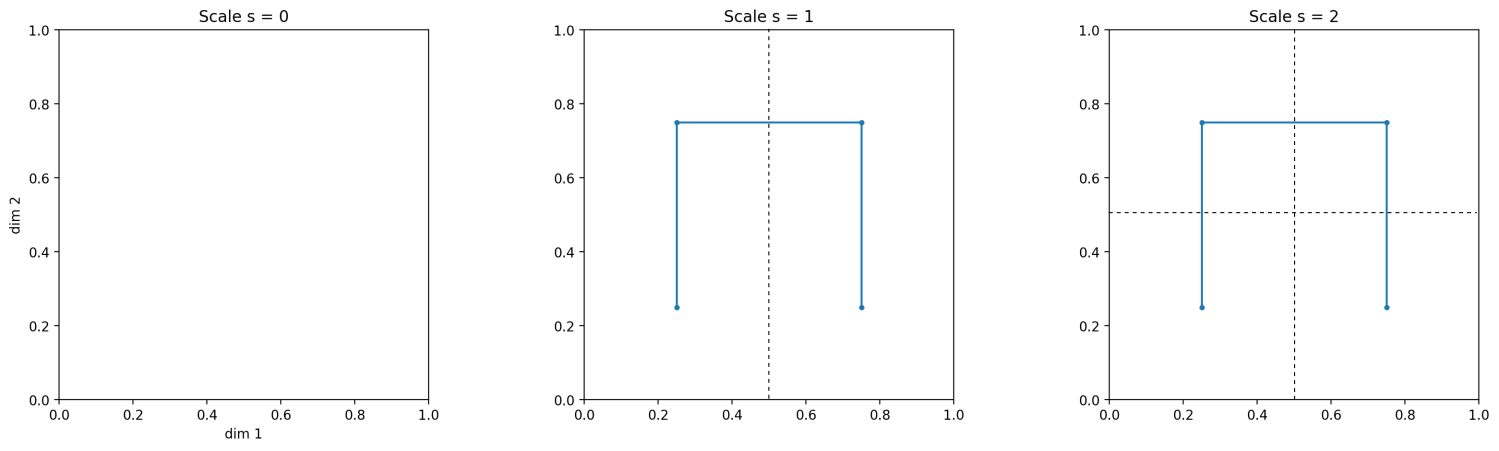
\includegraphics[trim={0 0 0 0}, clip, width=0.45\textwidth]{figures/partition_2d_top2.png}
            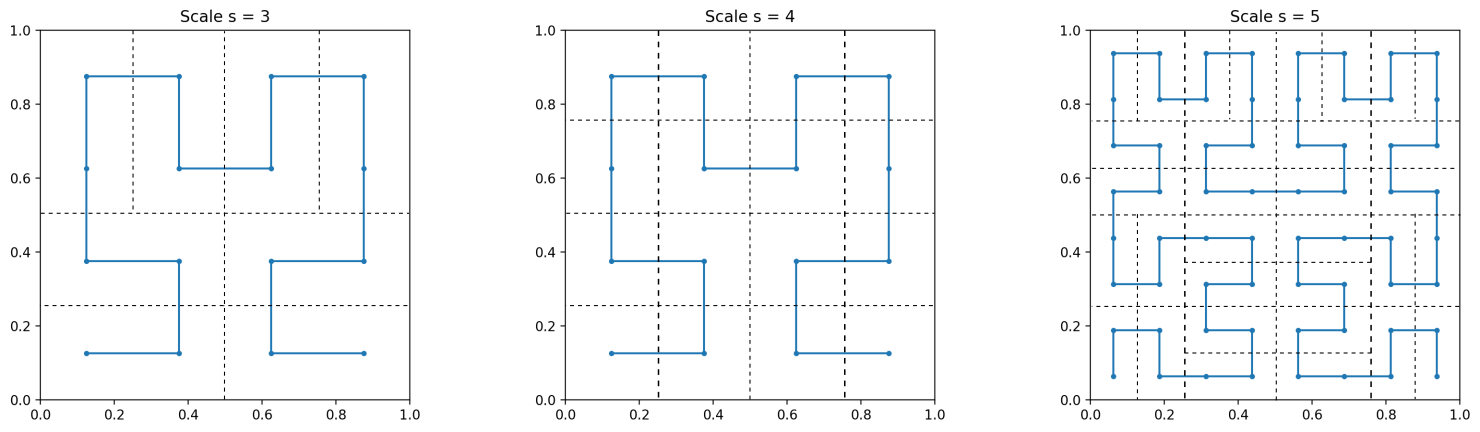
\includegraphics[trim={0 0 0 0}, clip, width=0.45\textwidth]{figures/partition_2d_bot2.png}
            \captionof{figure}{Dyadic partition of $[0,1]^2 $ obtained by the application of the Hilbert curve, for $ s = 1, \ldots, 5$.
            }
            \label{fig:partition-2d}
        \end{center}

        Sampling at each node from $ G_0$ truncated to $ \Theta_{\bm{\mu}; s,h}$ yields the \textbf{prior for the location parameter},
        \[
            \bm{\mu}_{s,h} \sim G_0 \cdot \one_{\Theta_{\bm{\mu};s, h}}.
        \]
        
        
        The scale parameters $ \Omega_{s,h}$ are sampled from a distribution $ H_0$ \textbf{scaled by a deterministic monotone decreasing sequence} in $ s$,
        \[
                        \Omega_{s,h} = \diag \big( c(s), \ldots, c(s) \big) W_{s,h}, \quad W_{s,h} \iid H_0.
        \]
\end{itemize}

%##########################################################
\color{DarkRed}
\section*{Interpretation}
\label{prop}
\color{Black}
%##########################################################

\begin{itemize}
\item Nodes higher in the tree correspond to \textbf{coarser kernels} whereas deeper nodes correspond to \textbf{more localized kernels}.
    The posterior adapts the kernels to the smoothness of the data.
\item We generalize a property of \citet{stefanucci2021} to show that the random location measure $G = \sum_{s=0}^{\infty }\sum_{h=1}^{2^s} \pi_{s,h} \delta_{\bm{\mu}_{s,h}}$ is \textbf{centered around $ G_0$} \textit{a priori},
    \[
        \mathbb{E}[G(A)] = G_0(A)\quad \text{for all $ A \subseteq \Theta_{\bm{\mu}}$}.
    \]
    
\item Also, we have control on the \textbf{prior average depth} of the binary tree by solving a 

\end{itemize}
\color{DarkRed}
\vspace{-0.3cm}

\color{DarkRed}
\section*{Performance in simulated datasets}
\color{Black}
We use the multiscale model with Gaussian prior on the location parameters and inverse Wishart prior on the scale parameter to have efficient Gibbs sampling updates \citep{kalli2011}.
\begin{itemize}
\item Scenarios: 1) mixture of normals/skew normals, 2) multiscale mixture.
\item Competitor: Pitman-Yor mixture model.
\item Mean posterior predictive distribution for the multiscale model in Figure~\ref{fig:ppd}.
\end{itemize}

\begin{center}\vspace{1cm}
    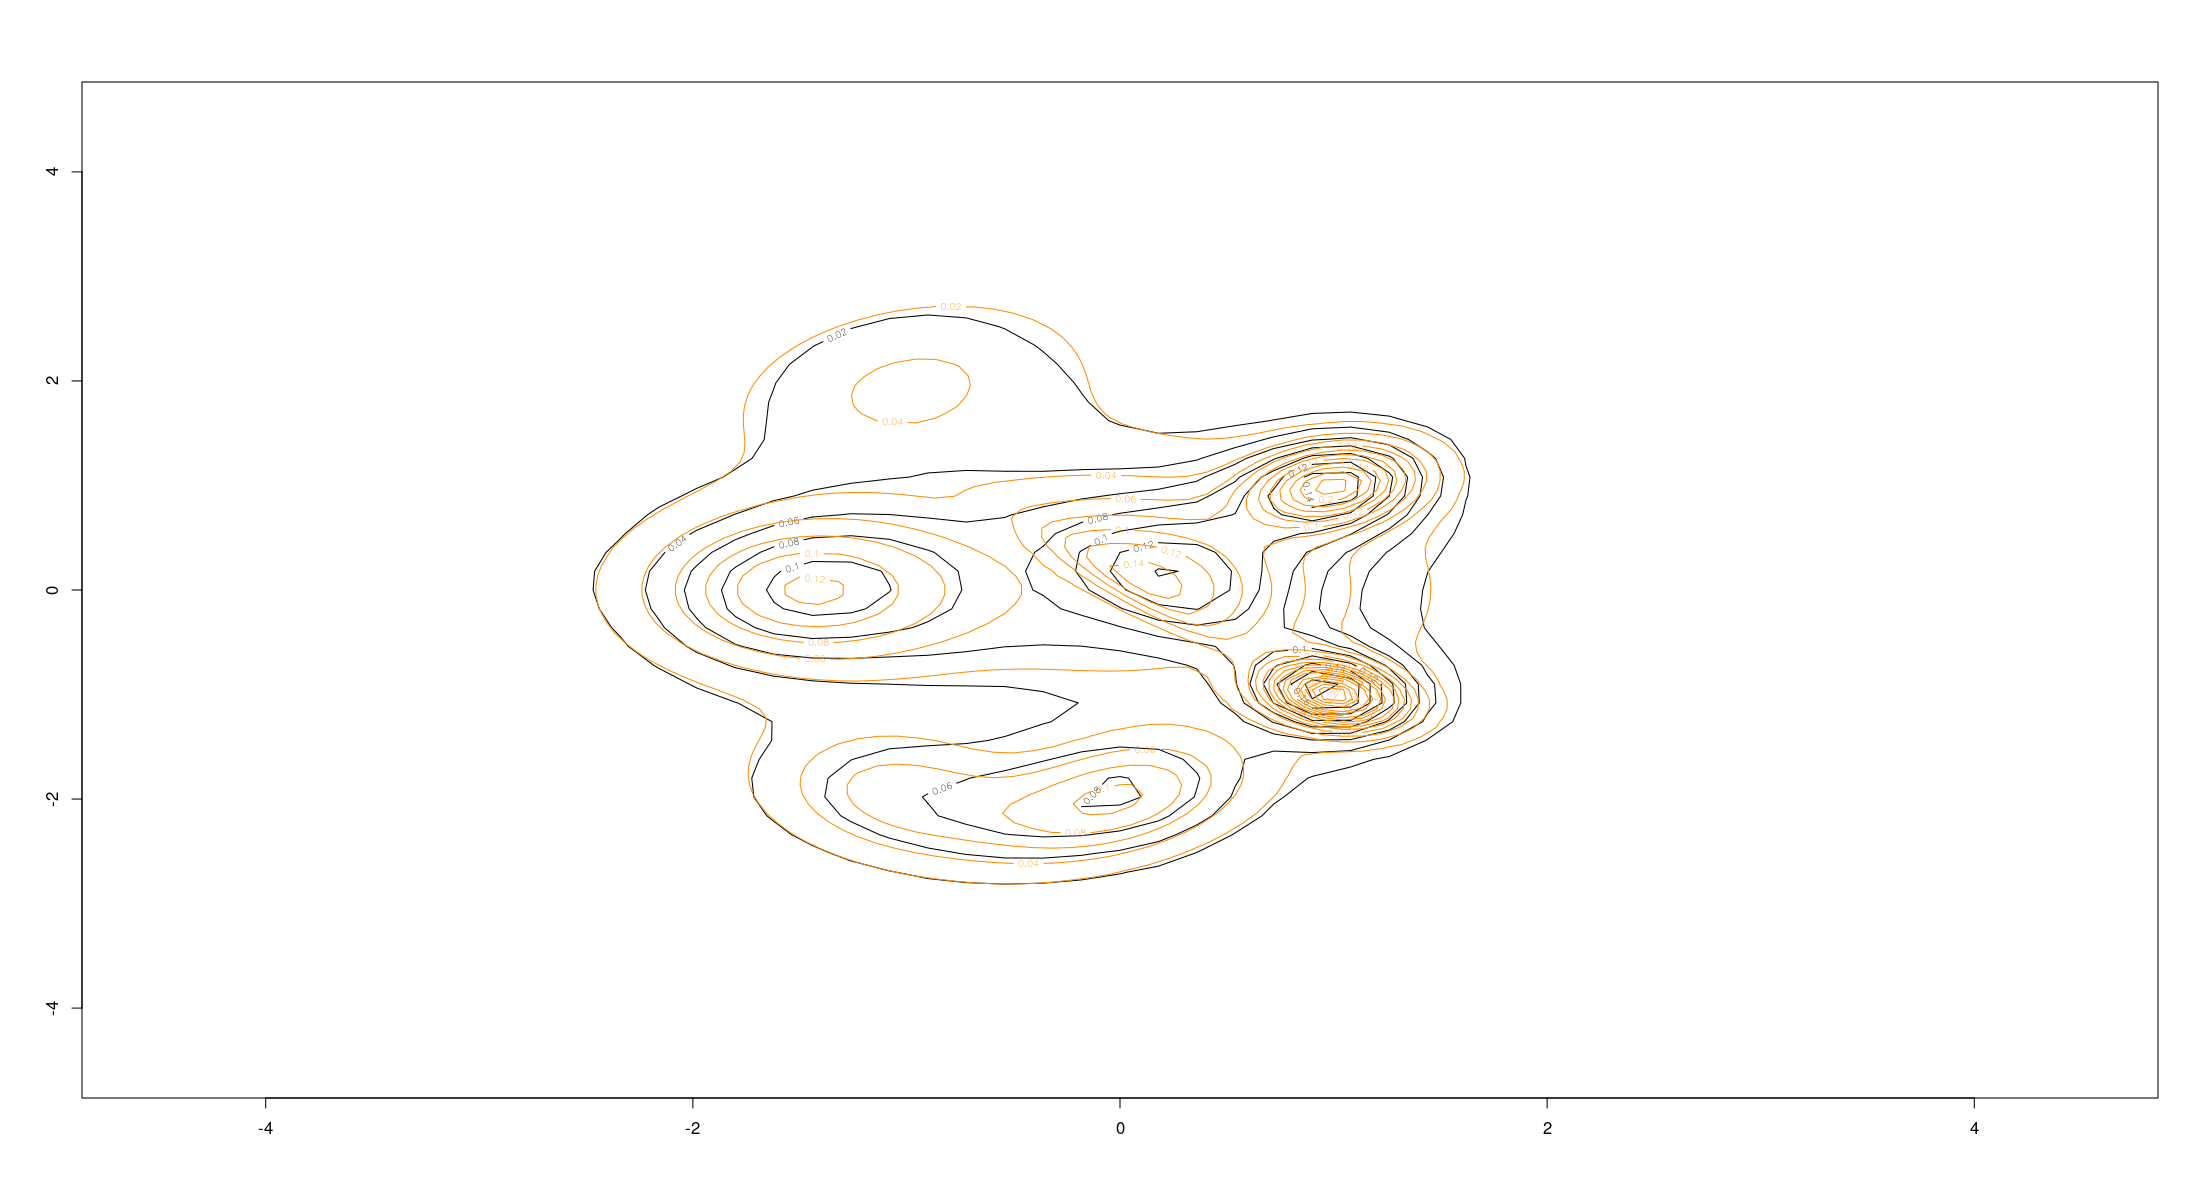
\includegraphics[width=0.225\textwidth]{r10average_ppdSmooth-indFALSE-red.png}
    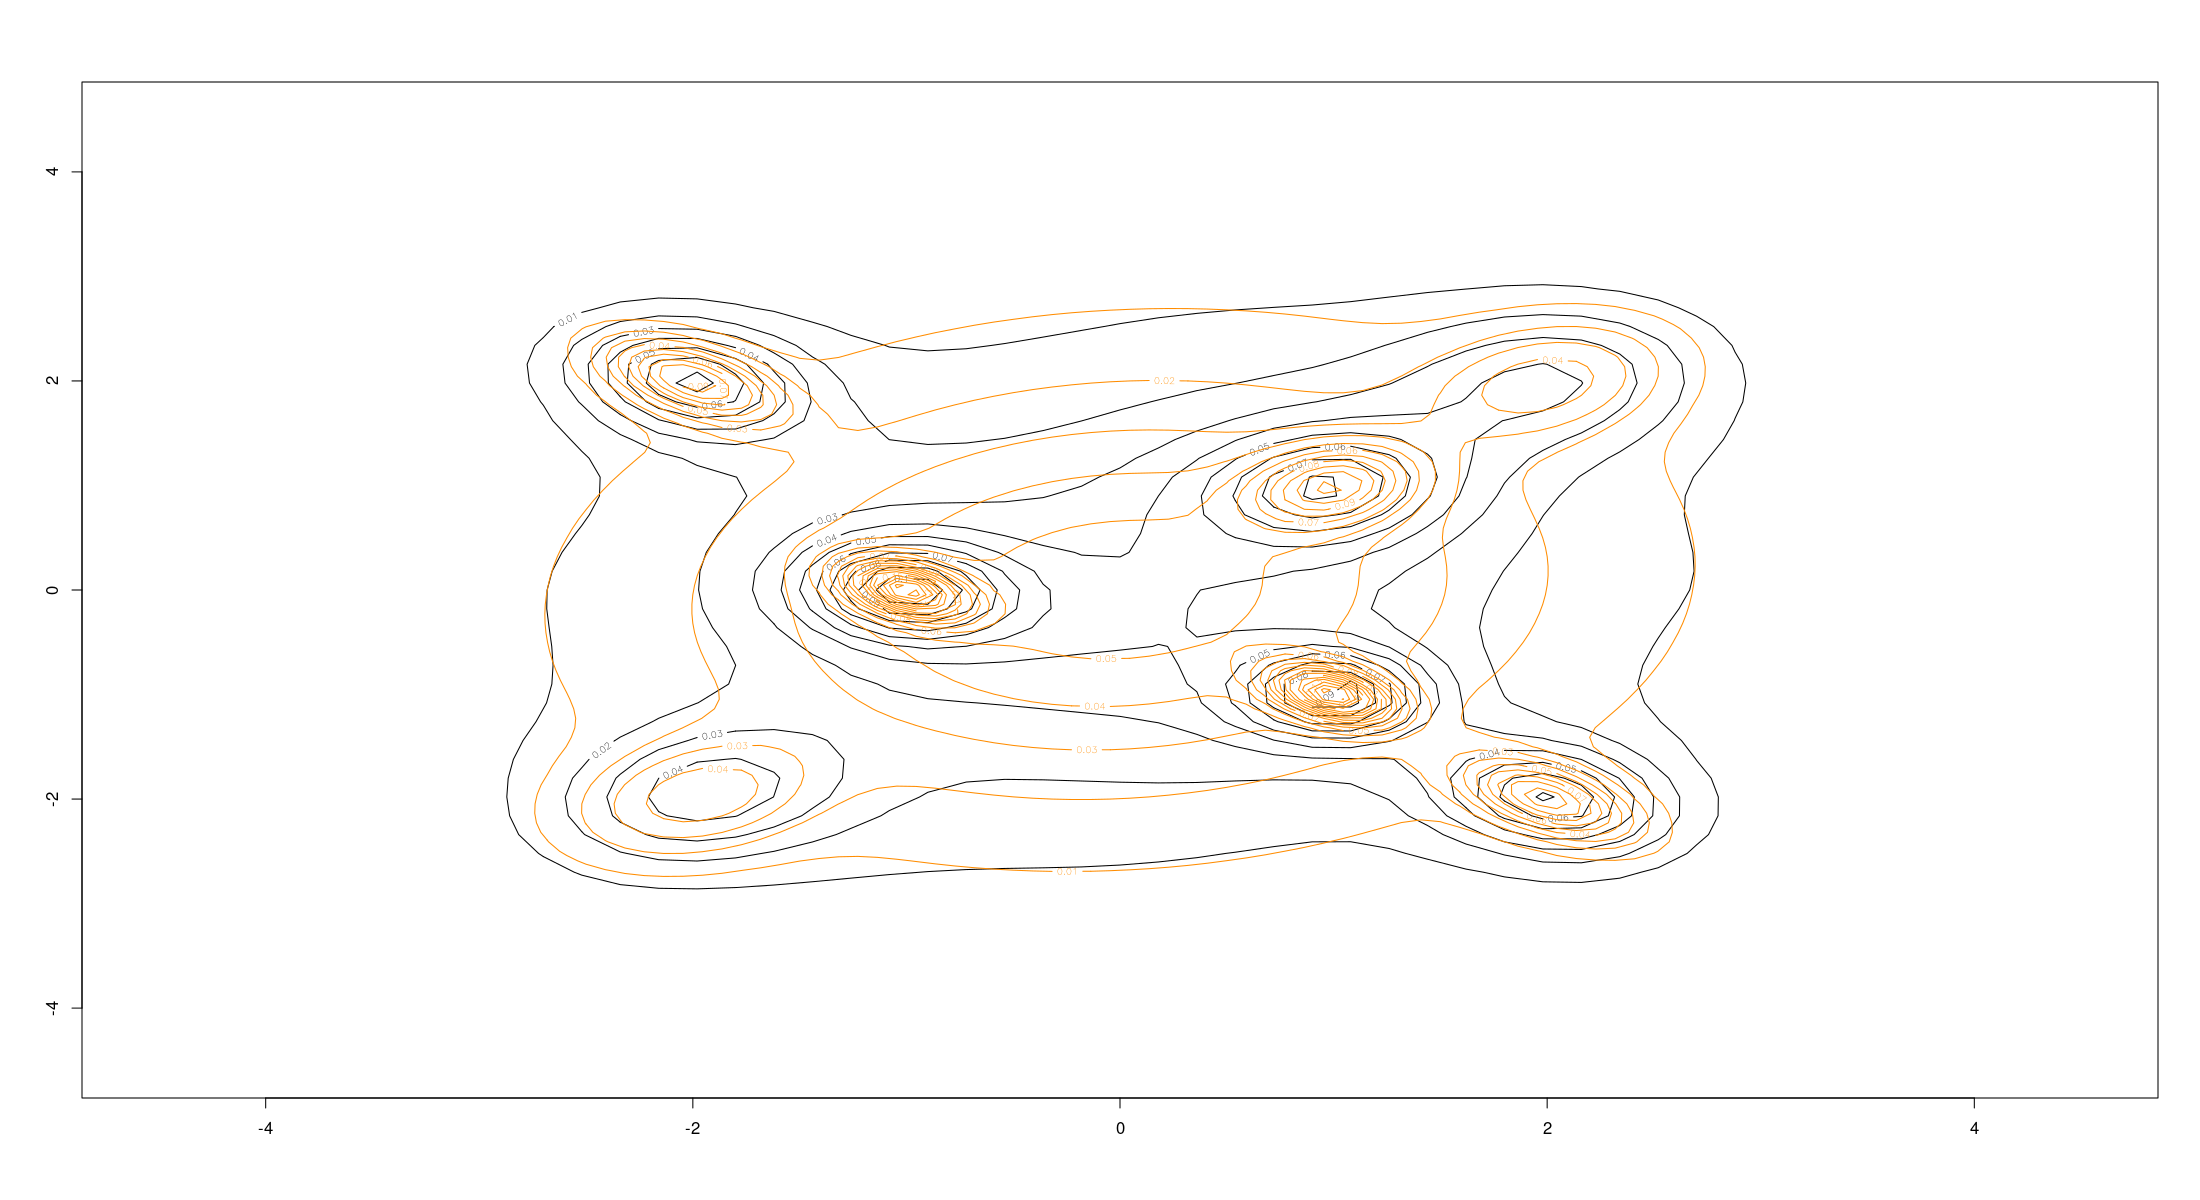
\includegraphics[width=0.225\textwidth]{r11average_ppdSmooth-indFALSE-red.png}

    \captionof{figure}{\label{fig:ppd} True density function (\textit{black}) and mean posterior predictive distribution (\textit{orange}) for the multiscale model.}
\end{center}

\begin{center}
    
\end{center}

\vspace{-1cm}

%##############-####################################################
\color{DarkRed}
\section*{Application to the Galaxy dataset}
\label{cpp}
\color{Black}

%##############-####################################################

\begin{itemize}
    \item The galaxy marginal distributions (Figure~\ref{fig:galaxy marginals}) are correctly estimated, except for the redshift which seems more problematic.

    \item The binary tree with nodes proportional to the estimated posterior median weight distribution (Figure~\ref{fig:galaxy binary tree}) gives \textbf{information} on the \textbf{location of the clusters within the space}.
    
\end{itemize}

\begin{minipage}[c]{0.45\textwidth}
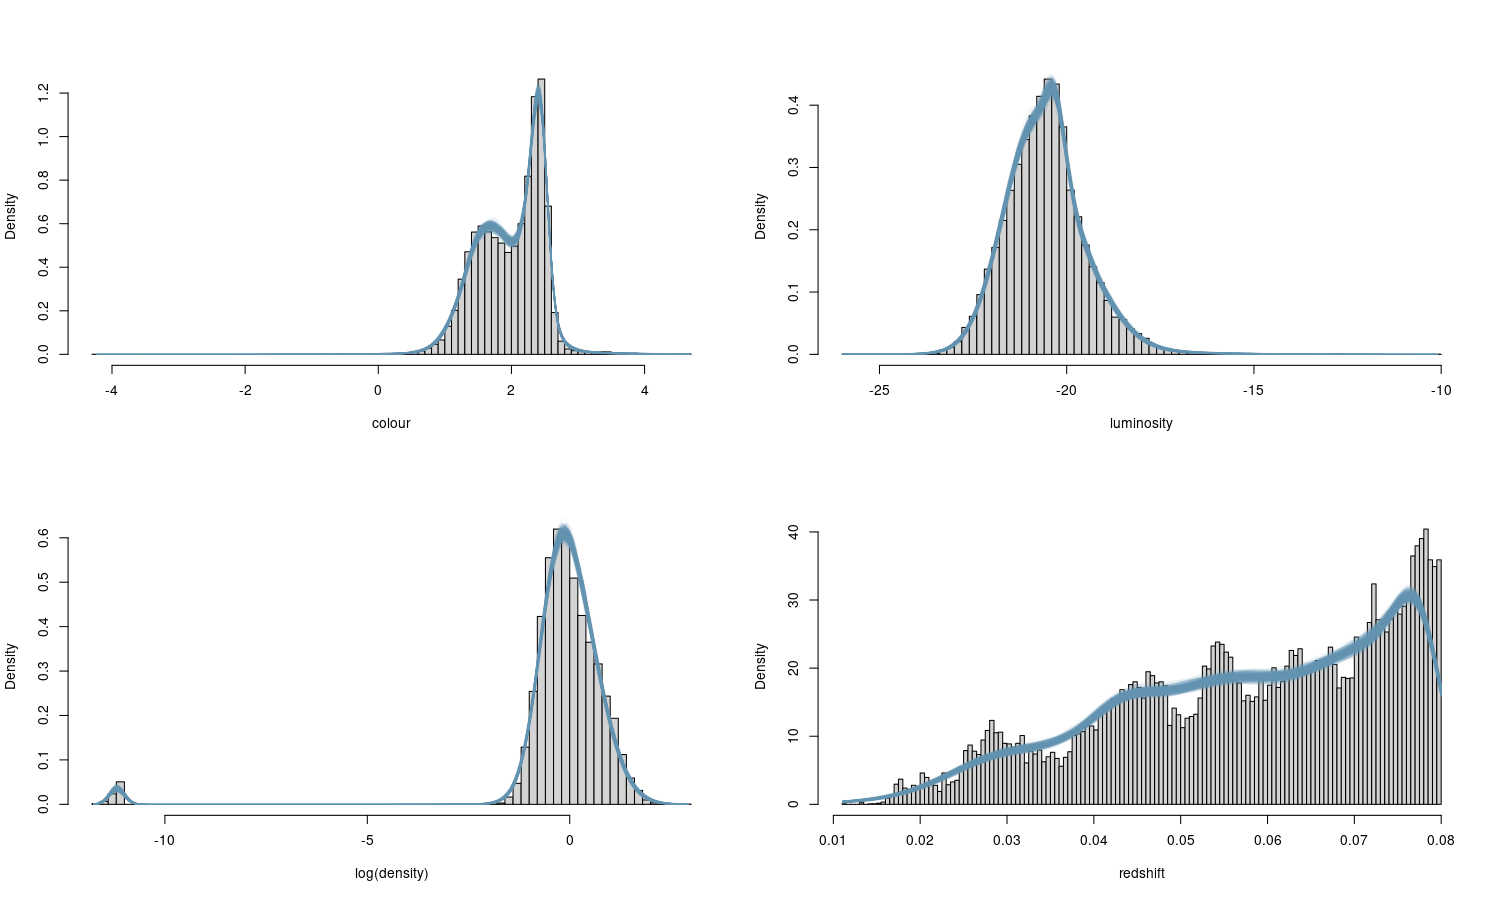
\includegraphics[width=1\textwidth]{posterior-predict-FALSE.png}
\captionof{figure}{\label{fig:galaxy marginals} Posterior predictive distribution for the marginal distributions of the Galaxy dataset.}
\end{minipage}

\begin{minipage}[c]{0.45\textwidth}
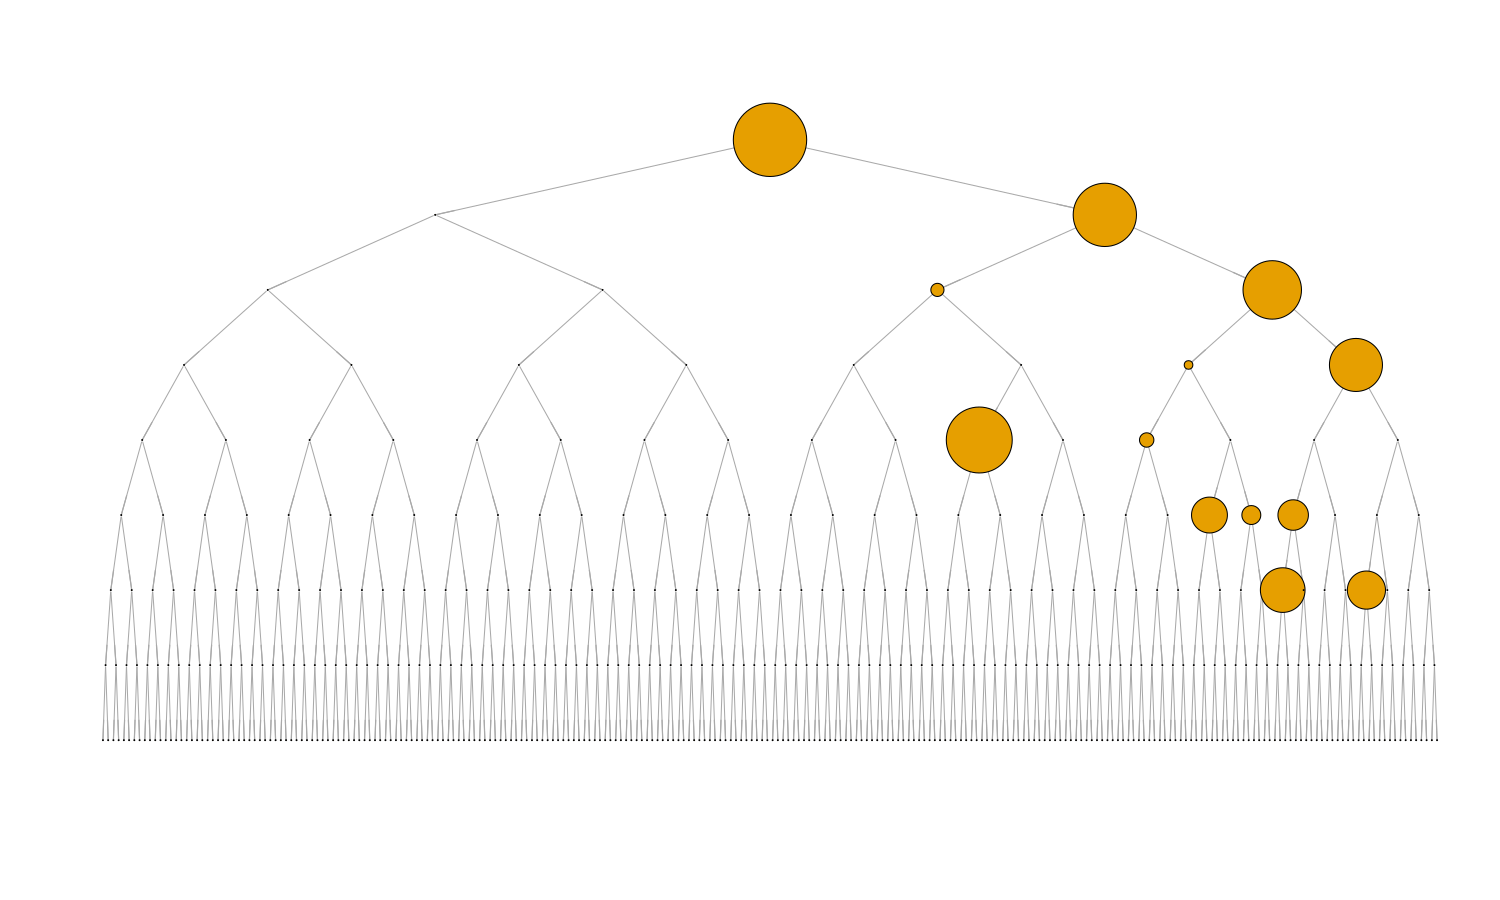
\includegraphics[width=1\textwidth]{binary-tree-FALSE.png}
\vspace{-4cm}
\captionof{figure}{\label{fig:galaxy binary tree} Multiscale binary tree with circles drawn proportionally to the median of the posterior distribution of the weights $ \pi_{s,h}$.}
\end{minipage}
%


\end{multicols} 


 %----------------------------------------------------------------------------------------
%	REFERENCES
%----------------------------------------------------------------------------------------
\mbox{}\\[0.5cm]
\begin{minipage}[t]{0.04\linewidth}
\centering
\mbox{}
\end{minipage}
\mbox{}
\begin{minipage}[t]{0.85\linewidth}
\bibliographystyle{plainnat}
\bibliography{biblio}
\end{minipage}

\end{document}
